\documentclass[a4paper,14pt]{article}
\usepackage{extsizes}
\usepackage{amsmath}
\usepackage{amssymb}
\everymath{\displaystyle}
\usepackage{geometry}
\usepackage{fancyhdr}
\usepackage{multicol}
\usepackage{graphicx}
\usepackage[brazil]{babel}
\usepackage[shortlabels]{enumitem}
\usepackage{cancel}
\columnsep=2cm
\hoffset=0cm
\textwidth=8cm
\setlength{\columnseprule}{.1pt}
\setlength{\columnsep}{2cm}
\renewcommand{\headrulewidth}{0pt}
\geometry{top=1in, bottom=1in, left=0.7in, right=0.5in}

\pagestyle{fancy}
\fancyhf{}
\fancyfoot[C]{\thepage}

\begin{document}
	
	\noindent\textbf{7FMA156~-~Matemática} 
	
	\begin{center}Interpretando textos e gráficos (Versão estudante)
	\end{center}
	
	
	\noindent\textbf{Nome:} \underline{\hspace{10cm}}
    \noindent\textbf{Data:} \underline{\hspace{4cm}}
	
	%\section*{Questões de Matemática}
	
	\begin{multicols}{2}
		Texto para as questões de 1 a 3: \\\\
		Os gráficos abaixo mostram, em milhões de reais, o total de vendas mensal que uma empresa realizou em 2018 e 2019 \\\\
		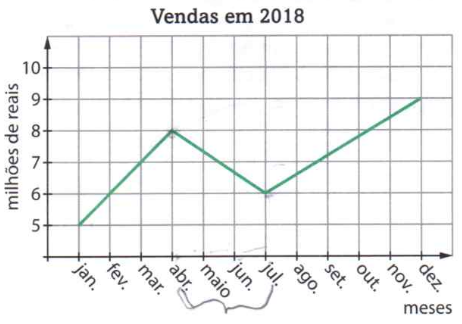
\includegraphics[width=0.45\textwidth]{/home/hogdelta/Documentos/latex/7FMA156_imagens/pg72-1.png} \\
		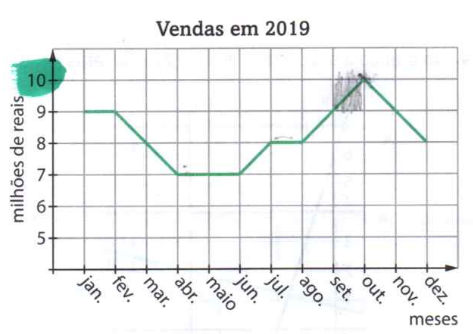
\includegraphics[width=0.45\textwidth]{/home/hogdelta/Documentos/latex/7FMA156_imagens/pg72-2.png}
		\begin{enumerate}
			\item Em qual período houve um decréscimo nas vendas de 2018? 
			\\\\\\\\\\\\\\
			\item Em 2019, após um decréscimo nas vendas, a empresa resolveu alterar sua estratégia em abril. Qual foi o mês em que esta empresa atingiu o máximo de vendas após esta estratégia? E qual foi o valor das vendas, em milhões de reais que a empresa realizou neste mês? 
			\\\\\\\\\\\\\\\\\\\\\\
			\item Qual foi, em milhões de reais o mínimo e o máximo de vendas realizadas pela empresa em 2018 e 2019?
			\\\\\\\\\\\\\\\\\\\\\\
			\item (ENEM) o gráfico abaixo mostra a área desmatada da Amazônia em km², a cada ano, no período de 1988 a 2008. \\
			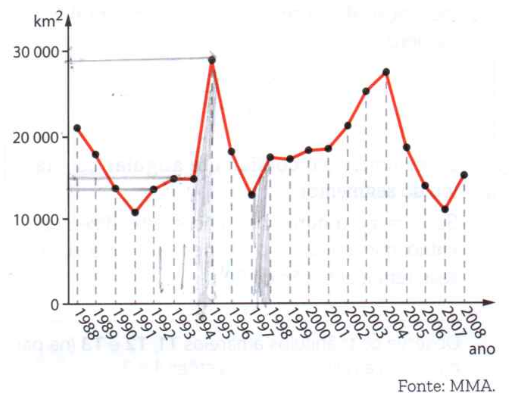
\includegraphics[width=0.45\textwidth]{/home/hogdelta/Documentos/latex/7FMA156_imagens/pg72-3.png}
		    \\
		    \begin{enumerate}[a)]
		    	\item As informações do gráfico indicam que:
		    	
		    	\item O maior desmatamento ocorreu em 2004.
		    	
		    	\item A área desmatada foi menor em 1997 que em 2007.
		    	
		    	\item A área desmatada a cada ano manteve-se constante entre 1998 e 2001.
		    	
		    	\item Área desmatada por ano foi maior entre 1994 e 1995 que entre 1997 e 1998.
		    	
		    	\item O total de área desmatado em 1992,993 e 1994 é maior que 60 000 km².
		    \end{enumerate}
			\item Com os dados do senso demográfico de 2000, apresentados no gráfico a seguir pode-se constatar que a redução da taxa de analfabetismo no Brasil é uma tendência que já vem sendo seguida desde a década de 1940. Observe que, a partir de 1980 (quando essa taxa foi de 26\%), essa redução é representada por um gráfico linear.
			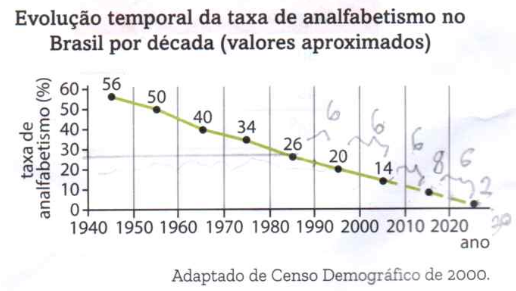
\includegraphics[width=0.45\textwidth]{/home/hogdelta/Documentos/latex/7FMA156_imagens/pg72-4.png} \\
			Supondo que essa tendência se mantenha, em que ano a taxa de analfabetismo no Brasil será exatamente igual a 5\%?
			\begin{enumerate}[a)]
				\item 2013. 
				\item 2014. 
				\item 2015. 
				\item 2016. 
				\item 2017.
			\end{enumerate}
		    \item Observe o gráfico a seguir. \\
		    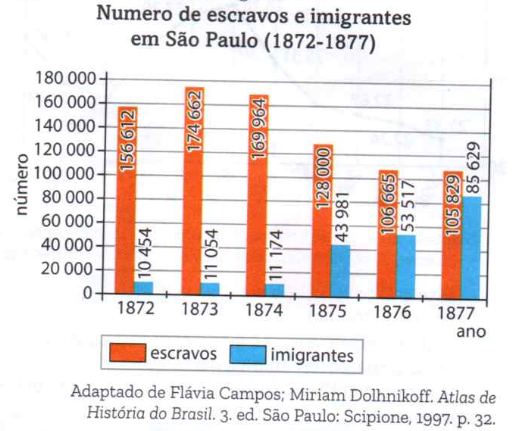
\includegraphics[width=0.45\textwidth]{/home/hogdelta/Documentos/latex/7FMA156_imagens/pg85-3.png} \\
		    Com base na análise desse gráfico, é correto afirmar que a razão entre o número de escravos e o número de imigrantes é:
		    \begin{enumerate}[a)]
		    	\item Constante no período de 1875 a 1877.
		    	\item Crescente no período de 1872 a 1877.
		    	\item Decrescente no período de 1872 a 1877.
		    	\item Decrescente no período de 1874 a 1877.
		    	\item Constante no período de 1873 a 1875.
		    \end{enumerate}
	        \item O tempo que um ônibus gasta para ir do ponto inicial ao ponto final de uma linha varia, durante o dia, conforme as condições do trânsito demorando mais nos horários de maior movimento. A empresa que opera essa linha forneceu, no gráfico a seguir, o tempo médio de duração da viagem conforme o horário de saída do ponto inicial, no período da manhã. \\
	        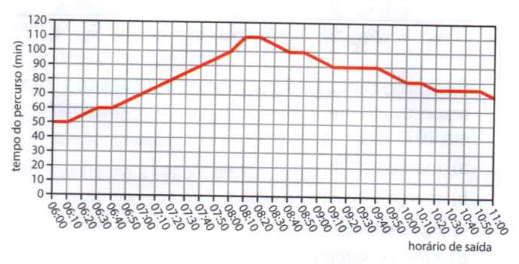
\includegraphics[width=0.45\textwidth]{/home/hogdelta/Documentos/latex/7FMA156_imagens/pg85-4.png}
	        De acordo com as informações do gráfico, um passageiro que necessita chegar até às 10h30min ao. Dessa linha deve tomar o ônibus no ponto inicial, no máximo, até as:
	        \begin{enumerate}[a)]
	        	\item 9h20min
	        	\item 9h30min
	        	\item 9h
	        	\item 8h30min
	        	\item 8h50min
	        \end{enumerate}
            \item O termo “agronegócio” não se refere apenas a agricultura e a pecuária, pois as atividades ligadas a essa produção inclui fornecedores de equipamentos, serviços para a zona rural, e industrialização e comercialização dos produtos. O gráfico seguinte mostra a participação percentual do agronegócio no PIB brasileiro: \\
            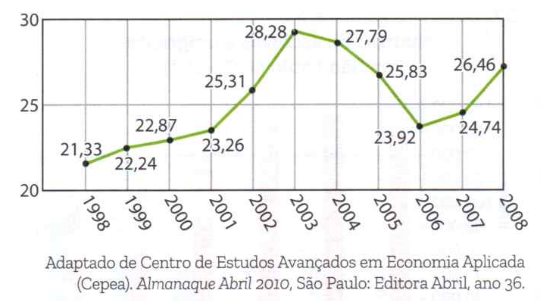
\includegraphics[width=0.45\textwidth]{/home/hogdelta/Documentos/latex/7FMA156_imagens/pg86-1.png} \\
            Esse gráfico foi usado em uma palestra na qual o orador ressaltou uma queda da participação do agronegócio no PIP brasileiro e a posterior recuperação dessa participação, em termos percentuais. \\
            Segundo o gráfico o período de queda ocorreu entre os anos de: \\
            \begin{enumerate}[a)]
            	\item 1998 e 2001.
            	\item 2001 e 2003.
            	\item 2003 e 2006.
            	\item 2003 e 2007.
            	\item 2003 e 2008.
            \end{enumerate}
            \item (ENEM) o dono de uma farmácia resolveu colocar a vista do público o gráfico mostrado a seguir, que apresenta a evolução do total de vendas (em reais) de certo medicamento ao longo do ano de 2011. \\
            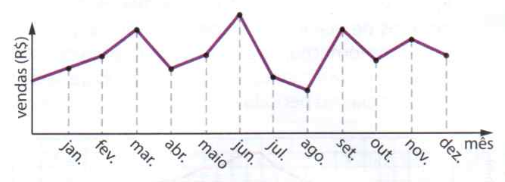
\includegraphics[width=0.45\textwidth]{/home/hogdelta/Documentos/latex/7FMA156_imagens/pg86-2.png} \\
            De acordo com o gráfico, os meses em que ocorreram, respectivamente, maior e a menor venda absolutas em 2011 foram:
            \begin{enumerate}[a)]
            	\item Março e Abril.
            	\item Março e agosto.
            	\item Agosto e setembro.
            	\item Junho e setembro.
            	\item Junho e agosto.
            \end{enumerate} 
		\end{enumerate}
	$~$ \\ $~$ \\ $~$ \\ $~$ \\ $~$ \\ $~$ \\ $~$ \\ $~$ \\ $~$ \\ $~$ \\ $~$ \\ $~$ \\ $~$ \\ $~$ \\ $~$ \\ $~$ \\ $~$ \\ $~$ \\ $~$ \\ $~$ \\ $~$ \\ $~$ \\ $~$ \\ $~$ \\ $~$ \\ $~$ \\ $~$ \\ $~$ \\ $~$ \\ $~$ \\ $~$ \\ $~$ \\ $~$ \\ $~$ \\ $~$ \\ $~$ \\ $~$ \\ $~$ \\ $~$ \\ $~$ \\ $~$ \\ $~$ \\ $~$ \\ $~$ \\ $~$ \\ $~$ \\ $~$ \\ $~$ \\ $~$ \\ $~$ \\ $~$ \\ $~$ \\ $~$ \\ $~$ \\ $~$ \\ $~$ \\ $~$ \\ $~$ \\ $~$ \\ $~$ \\ $~$ \\ $~$ \\ 
    \end{multicols}
\end{document}









